\chapter{Implementação do Ambiente de DWing}
\label{estudo de caso}

\section{Arquitetura da Implementação}

Para a implementação do ambiente do DWing para métricas de código-fonte, foi definida a arquitetura tal como se mostra Figura \ref{arquitetura}.


\begin{figure}[ht!]
\centering
\includegraphics[keepaspectratio=false,scale=0.20]{figuras/arquitetura-dwing.eps}
\caption{Arquitetura do Ambiente de DWing para Métricas de Código-Fonte}
\label{arquitetura}
\end{figure}
\FloatBarrier

Para selecionar as ferramentas, que implementarão cada um dos componentes do ambiente DWing, estabeleceram-se critérios gerais de seleção tal como pode ser visto na Tabela \ref{seleção}.


	\begin{table}[!ht]
	\begin{center}
	 \begin{tabular}{|l|l|}
		\hline
		Identificador & Critério 
		\\ \hline
		CG01 & A ferramenta deve possuir código aberto.  
		\\ \hline
		CG02 & A ferramenta deve ter documentação disponível em inglês ou português.      
		\\ \hline
		CG03 & A ferramenta deve possuir uma comunidade ativa em seu uso.
		\\ \hline
		CG04 & A ferramenta deve possuir releases estáveis.    
		\\ \hline
		\end{tabular}
		\caption{Critérios Gerais de seleção de ferramentas}
		\label{seleção}
		\end{center}
		\end{table}	


\section{Ferramenta de Análise Estática de Código-Fonte}

Além dos critérios gerais estabelecidos, para escolha da ferramenta de análise estática de código-fonte, que são as fontes externas de coleta, estabeleceram-se os critérios específicos para seleção de ferramentas de análise estática de código fonte (CAE) apresentados na Tabela \ref{specific}


	\begin{table}[!ht]
	\begin{center}
	 \begin{tabular}{|l|p{10cm}|}
		\hline
		Identificador & Critério 
		\\ \hline
		CAE01 & A ferramenta deve prover as métricas de código-fonte para as linguagens de programação, tal como especificado na Tabela \ref{metrics}.
		\\ \hline
		CAE02 & A ferramenta deve possuir saída de dados em arquivo em alguns dos seguintes formatos: JSON, XML, TXT, CSV.      
		\\ \hline
		CAE03 & A ferramenta deve ser mutiplataforma.
		\\ \hline
		\end{tabular}
		\caption{Critérios Específicos para Ferramenta de Análise Estática de Código-Fonte}
		\label{specific}
		\end{center}
		\end{table}	

Após a realização de uma busca por ferramentas de análise estática de código-fonte, foram pre-selecionados o SonarQube~\footnote{Disponível em \url{http://www.sonarqube.org/}} e Analizo~\footnote{Disponível em \url{http:/http://analizo.org/}} cujas principais características de ambas são apresentadas na Tabela \ref{dados-ferramentas-estatica}.

\begin{savenotes}
\begin{table}[!ht]
\centering
\begin{tabular}{|p{5cm}|p{4.5cm}|p{5cm}|}
\hline

Característica 

&

\begin{center}

\includegraphics[keepaspectratio=false,scale=0.48]{figuras/analizo.eps} 
\end{center}


&



\begin{center}

\includegraphics[keepaspectratio=false,scale=0.48]{figuras/sonarqube.eps} 
\end{center}





   
\\ \hline


%--------------------------
Linguagens com Suporte  & C, C++, Java & C, C++, Java, PHP,Scala, Python, Delphi, Pascal, Flex, ActionScript, Javascript, Groovy~\footnote{O SonarQube oferece suporte comercial a outras linguagens, contudo foram listadas apenas que tem suporte por meio de \textit{plugins} de código-aberto} \\ \hline
Licença  & GNU GPL3 & GNU LGPL3  \\ \hline



%-----------------------------------

Métricas de Código-Fonte fornecidas  & 9 métricas em âmbito de Projeto e 16 métricas em âmbito de Classe \cite{Meirelles2013} & 12 métricas em âmbito de Classe, 8 métricas em âmbito de projeto. \\ \hline


%--------------------------
Formato de Saída das Métricas  & YAML & JSON, XML \\ \hline

%--------------------------
Plataforma  &Windows, Linux, Mac OS X e Servidores de Aplicação Java & Debian e Ubuntu                                                                                              \\ \hline

%--------------------------
Integração com outras ferramentas & Mezuro, Kalibro & Jenkins, Hudson, Mantis, JIRA, Crowd e entre outros \\ \hline

%--------------------------
\multirow{4}{5cm}{Números do Repositório Oficial no GitHub em 14/11/2013}
& \textit{Commits:} 639  & \textit{Commits:} 7532\\ \cline{2-3} 

&\textit{Branches:} 1 & \textit{Branches:} 16  \\ \cline{2-3} 
& Contribuidores: 7 & Contribuidores: 18 \\ \cline{2-3} 
& \textit{Releases:} 27  & \textit{Releases:} 36

 \\ \hline

%--------------------------
Número de Casos Abertos no \textit{Issue Tracker} em 14/11/2013 & 26  & 552  
\\ \hline

%--------------------------
Sistema de Controle de Versões & Git & Git \\ \hline

%--------------------------
Idioma com Suporte & Inglês & Inglês, Português, Japonês, Italiano, Chinês, Francês, Grego e Espanhol \\ \hline

%------------------------
Idioma da Documentação & Inglês & Inglês

\\ \hline
%-----------------------
Última Versão Estável em 14/11/2013 & 1.17.0 & 4.0  

\\ \hline
 %-----------------------
Data de Lançamento da Última Versão Estável & 31 de Janeiro de 2013 & 4 de Novembro de 2013

\\ \hline
\end{tabular}
\caption{Características do SonarQube e do Analizo}
\label{dados-ferramentas-estatica}
\end{table}
\FloatBarrier
\end{savenotes}

Tendo as características gerais de cada ferramenta levantadas, foram comparadas (SonarQube e Analizo) quanto aos critérios gerais e aos critérios específicos para ferramentas de análise estática, tal como se mostra na Tabela \ref{compare}.


\begin{table}[!ht]
\centering
\begin{tabular}{|l|l|l|}
\hline
Critérios & SonarQube  & Analizo    \\ \hline
CG01      & \checkmark & \checkmark \\ \hline
CG02      & \checkmark & \checkmark \\ \hline
CG03      & \checkmark & \checkmark \\ \hline
CG04      & \checkmark & \checkmark \\ \hline
CAE01     & \checkmark & \checkmark \\ \hline
CAE02     & \checkmark & \checkmark \\ \hline
CAE03     & \checkmark & \xmark     \\ \hline
\end{tabular}
\caption{Análise do SonarQube e do Analizo quanto aos critérios gerais e quanto aos critérios específicos de ferramentas de análise estática}
\label{compare}
\end{table}
\FloatBarrier


Dado a comparação, percebe-se que ambas as ferramentas cumprem o próposito geral de levantar as métricas de código-fonte, com a diferença que SonarQube possui um suporte a mais linguagens de programação quando comparado com o Analizo, contudo dado que o escopo da análise de \citeonline{Meirelles2013} se restringe a Java e C++, logo a falta de suporte à outras linguagens que o SonarQube suporta não é fator excludente da utilização do Analizo.

Percebe-se, ainda devido aos critérios específicos de selação de ferramentas de análise estática, que o Analizo tem uma plataforma específica, sendo que o SonarQube é mutiplataforma. Contudo, entende-se que como há objetivo de construir um ambiente de \textit{Data Warehousing} utilizando ferramentas livres, logo poder-se-ia escolher também uma plataforma livre tal como o Ubuntu ou Debian.

A escolha foi ponderada então pelo formato de saída do arquivo. \citeonline{fonseca2007alternativas} realizou um estudo experimental entre XML, JSON (Formatos de Saída do SonarQube) e YAML (Formato de Saída do Analizo), que é mostrado na Figura \ref{jsonvsyaml}.

\begin{figure}[ht!]
\centering
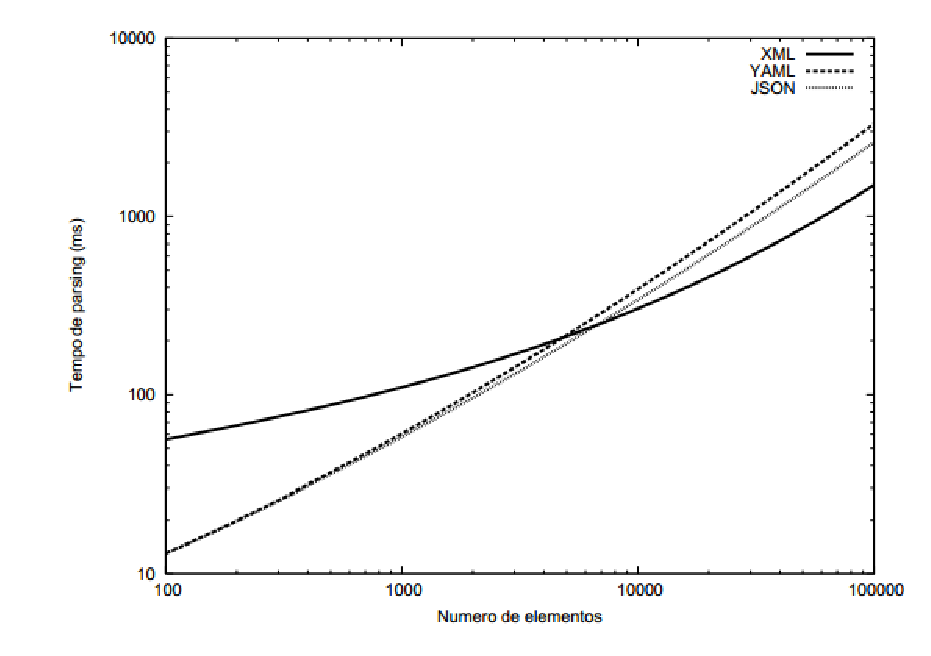
\includegraphics[keepaspectratio=false,scale=1]{figuras/json.eps}
\caption{Comparação entre JSON, YAML e XML extraído de \citeonline{fonseca2007alternativas}}
\label{jsonvsyaml}
\end{figure}
\FloatBarrier

Após a análise da Figura \ref{jsonvsyaml}, percebe-se que o YAML perde em desempenho para JSON e XML quando o número de elementos aumenta gradativamente. Em projetos de software, é natural que estes cresçam cada vez mais, tal como especifica a segunda lei de \citeonline{Lehman1980b}, logo o formato JSON ou XML é mais adequado, fazendo com que a ferramenta SonarQube seja mais indicada para o contexto deste trabalho.

Entre JSON e XML, \citeonline{fonseca2007alternativas} conclui que o transporte de dados é mais rápido utilizando JSON, pois se permite transportar
um objeto serializado arbitrariamente complexo, e transformá-lo num objeto
JavaScript sem grandes problemas, enquanto que o XML se deve construir um \textit{parser} para interpretar os dados. Por este motivo, foi escolhido para extração das métricas de código-fonte neste trabalho, o formato JSON provido pela ferramenta SonarQube. 


\subsection{Acompanhamento das Métricas de Código-Fonte de um Software Livre}

Com o objetivo de validar a implementação do ambiente de DWing para métricas de código-fonte, escolheu-se nesta etapa do trabalho de conclusão de curso, acompanhar a qualidade de um software livre conforme especificado pelo objetivo específico OE2.

Dado que os intervalos constituídos da análise de \citeonline{Meirelles2013}, apresentados na seção \ref{Intervalos das Métricas}, são para as linguagens de programação C++ e Java, há então a restritividade quanto ao acompanhamento de projetos feitos nessas linguagens.

Após uma leitura da documentação do SonarQube, descobriu-se que este mantém um repositório de análises de código-fonte de projetos de software livre, chamado Nemo~\footnote{Disponível em \url{http://nemo.sonarqube.org/}}. O Nemo disponibiliza projetos feitos nas linguagens Java, Javascript, Groovy e entre outros. Limitando-se apenas a linguagem Java, dado que não foi encontrado nenhum projeto C++ no repositório com grande frequência de atualizações, obteve-se cerca de 178 projetos.

A fim de se detectar projetos que tinham a maior taxa de atualização no repositório de análises do Nemo, percebeu-se que o projeto \textbf{Apache Maven} era um dos que mais se mantinham atualizados. Feito em linguagem Java, este projeto disponibiliza uma nova análise sobre o código-fonte a cada semana. Diante disso, foi escolhido o Apache Maven como o software a ser monitorado no ambiente de DWing. 




\section{Projeto do \textit{Data Warehouse}}

O \textit{Data Warehouse} como elemento central do ambiente de \textit{Data Warehousing} deve ser o primeiro a ser projetado \cite{Kimball2002}. Isso ocorre pois o DW deve ser dirigido ao negócio. Logo a modificação do DW impacta principalmente na carga dos dados, na etapa de extração, transformação e carga, requerendo modificações conforme o DW venha a mudar.

Seguindo a metolodogia proposta por \citeonline{Kimball2002}, apresentada na seção \ref{metodologia-dw}, entende-se que o processo de negócio deste trabalho de conclusão de curso, é avaliar a qualidade do código-fonte continuamente por meio das métricas de código-fonte. \citeonline{Kimball2002} enuncia que o segundo passo após a indentificação do processo de negócio, é a identificação da peridiociodade dos dados coletados pelo mesmo.


No processo de negócio de métricas de código-fonte, a periodicidade de coleta dos dados é variável, isto é, depende de projeto a projeto. Visando atender a maior parte dos casos possíveis, identificou-se a menor granuladidade para agregação: o dia. Isto ocorre, pois as ferramentas de integração contínua, que são muito utilizadas em ambientes ágeis \cite{beckarticle1999}, permitem a estabilização de um pacote de software por dia, logo a menor análise do código-fonte pode ser realizada sobre esse pacote estável diariamente. Contudo, há projetos que liberam versões estáveis com mais tempo, portanto se deve permitir agregações maiores tais como, mês, trimestre, semestre e ano. Para esta etapa do trabalho de conclusão de curso, optou-se pela implementação da agregação diária.


Seguindo os passos subsequentes da metodologia proposta por \citeonline{Kimball2002}, foram identificados as dimensões e o fato por meio da modelagem multidimensional, tal como mostra a Figura \ref{esquema}, utilizado a ferramenta MySQL Workbench~\footnote{Disponível em \url{http://dev.mysql.com/downloads/tools/workbench/}} que é um software de código aberto com licença GPL 2.0.


\begin{figure}[ht!]
\centering
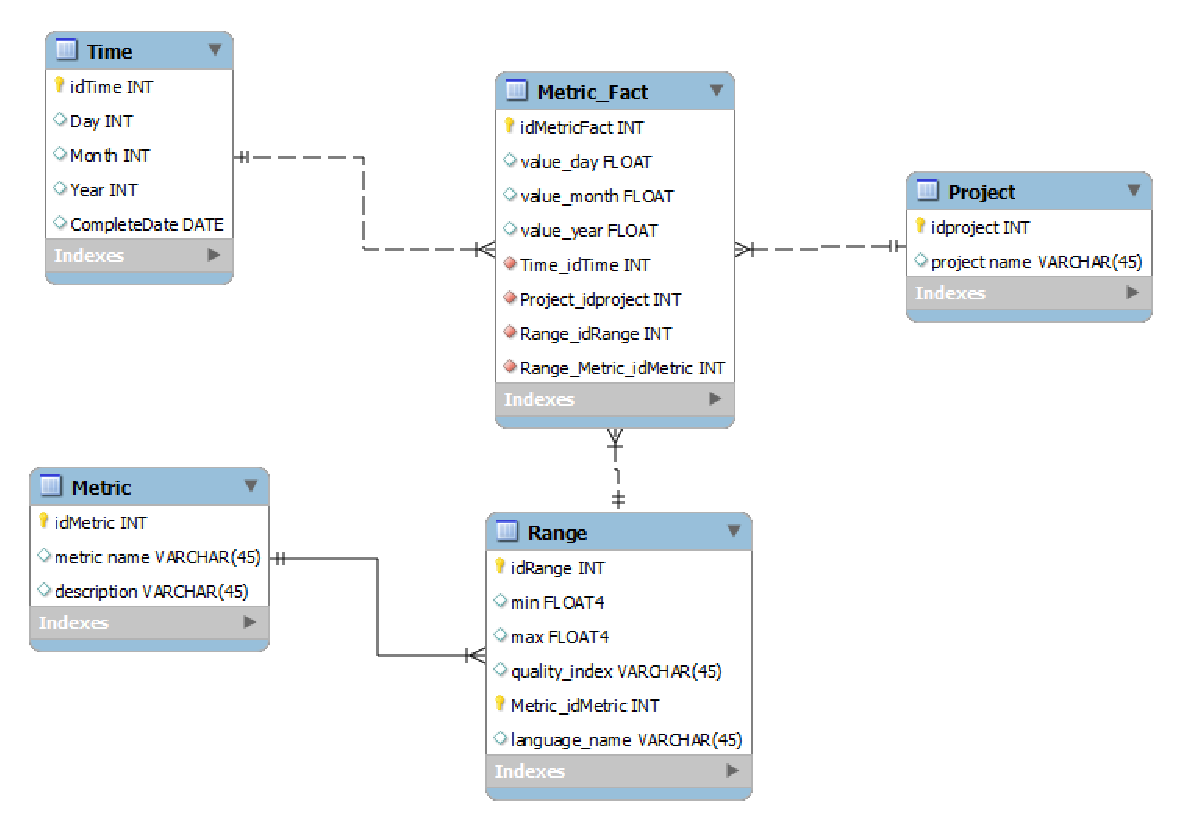
\includegraphics[keepaspectratio=false,scale=0.60]{figuras/esquema.eps}
\caption{Modelo Multidimensional do \textit{Data Warehouse}}
\label{esquema}
\end{figure}
\FloatBarrier

O modelo multidimensional, que tem seu SQL resultante apresentado no Apêndice \ref{sql-datawarehouse}, foi implementado no MySQL Community Server ~\footnote{Disponível em \url{http://dev.mysql.com/downloads/mysql/}} que também possui uma licença de código aberto GPL 2.0

Quanto ao fato (Metric\_Fact) é possível dizer que o mesmo é semi-aditivo, pois as métricas de código-fonte não podem ser somadas a nenhuma dimensão. Este fato é calculado por meio do 75º percentil na etapa de transformação dos dados, tal como explicado na seção \ref{Intervalos das Métricas}.


\section{Ferramentas de Dwing}

Tendo em vista que o \textit{Data Warehouse} foi projetado em um modelo dimensional, é possível construir tanto o processo de \textit{Extraction-Transformation-Load} quanto as operações de consulta OLAP. Entre as alternativas de código aberto que suportam este ambiente como um todo, está o Pentaho BI Suite Community Edition. Este apresenta soluções que cobrem 
as áreas de ETL, \textit{reporting}, OLAP e mineração de dados. Cada um dos componentes utilizados é apresentado e analisado nas seções subsequentes.
 


\subsection{Implementação da Extração, Transformação e Carga dos Dados}
\label{implementação-ETL}
O Pentaho Data Integration Community Edition ou Kettle\footnote{Disponível em \url{http://kettle.pentaho.com/}}, como é conhecido pela comunidade que o desenvolve, é feito na linguagem Java e implementa o processo de ETL (Extração, Transformação e Carga de Dados). A interface do Kettle é mostrada na Figura \ref{pdi} e as principais características do Kettle e a análise quanto aos critérios gerais de seleção de ferramentas são apresentadas na Tabela \ref{kettle}.

\begin{figure}[ht!]
\centering
\includegraphics[keepaspectratio=false,scale=0.45]{figuras/pdi.eps}
\caption{Interface do Kettle}
\label{pdi}
\end{figure}
\FloatBarrier
 

\begin{table}[!ht]
\begin{tabular}{|p{4.5cm}|p{5.0cm}|p{1cm}|p{1cm}|p{1cm}|p{1cm}|}
\hline
Característica                                          

&



\begin{center}

\includegraphics[keepaspectratio=false,scale=0.48]{figuras/kettle-logo.eps} 
\end{center}                                              

& CG01 

& CG02       

& CG03       


& CG04       


\\ \hline

Licença                                                 & Apache License 2.0                              & \checkmark &            &            &            \\ \hline
Integração com Banco de Dados                           & MySQL, SQLServer, PostgreSQL, Oracle entre outros &            &            &            &            \\ \hline
Formatos Aceitos de Entrada de Dados                    & XML, TXT, JSON, ODS, XLS, CSV, Tabelas, YAML    &            &            &            &            \\ \hline
Ultima Versão Estável (14/11/2013)                      & 4.4                                             &            &            &            & \checkmark \\ \hline
Quantidade de Commits no Repositório Oficial            & 10.000                                         &            &            & \checkmark &            \\ \hline
Idioma da Documentação                                  & Inglês                                          &            & \checkmark &            &            \\ \hline
Quantidade de Casos Abertos no \textit{Issue Tracker} & 2875                                           &            &            & \checkmark &            \\ \hline

\end{tabular}
\caption{Características do Kettle e avaliação quanto aos critérios gerais de seleção de ferramentas}
\label{kettle}
\end{table}
\FloatBarrier	

O Kettle possui dois tipos de componentes internos: \textit{Transformation} e \textit{Job}. O primeiro permite mover dados de uma origem até um destino, já a \textit{Transformation} permite executar tarefas, em nível mais alto, de fluxo de controle, tais como, mandar um email em caso de falha, baixar um arquivo, executar transformações  e entre outras atividades.

Para a implementação do ETL no Kettle, utilizou-se os arquivos resultantes da análise do SonarQube em JSON e conexão com o MySQL Server, onde foi implementado o Data Warehouse. As implementações detalhadas de \textit{Transformation} e \textit{Job} são apresentados no apêndice \ref{kettle-implementação}.


\subsection{Implementação das Consultas OLAP e Visualização de Dados}

Para a implementação das consultas OLAP e Visualização de dados, torna-se necessário a utilização do Pentaho BI Platform\footnote{Disponível em \url{http://community.pentaho.com/projects/bi_platform/}}, que é uma ferramenta provê a arquitetura e a infraestrutura para soluções de \textit{Business Inteligence}, \textit{Data Mining} e a camada de visualização de dados do \textit{Data Warehouse}.


O Pentaho BiPlatform, cuja interface inicial apresentada na Figura \ref{BIplatform}, tem as principais características e a análise quanto aos critérios gerais de seleção de ferramentas são apresentadas na Tabela \ref{biserver}. 


\begin{table}[!ht]
\begin{tabular}{|p{4.5cm}|p{5.0cm}|p{1cm}|p{1cm}|p{1cm}|p{1cm}|}
\hline
Característica                                          

&



\begin{center}

\includegraphics[keepaspectratio=false,scale=0.48]{figuras/pentaho_logo.eps} 
\end{center}                                              

& CG01 

& CG02       

& CG03       


& CG04       


\\ \hline

Licença                                                 & Apache License 2.0                              & \checkmark &            &            &            \\ \hline
Integração com Banco de Dados                           & MySQL, SQLServer, PostgreSQL, Oracle entre outros &            &            &            &            \\ \hline
Linguagem em que foi densenvolvida & Java &            &            &            &

 \\ \hline
Ultima Versão Estável (14/11/2013)                      & 4.8                                             &            &            &            & \checkmark \\ \hline
Quantidade de Commits no Repositório Oficial em 14/11/2013            & 3700                                         &            &            & \checkmark &            \\ \hline
Idioma da Documentação                                  & Inglês                                          &            & \checkmark &            &            \\ \hline
Quantidade de Casos Abertos no \textit{Issue Tracker} & 1489                                            &            &            & \checkmark &            \\ \hline

\end{tabular}
\caption{Características do Pentaho BI Platform e avaliação quanto aos critérios gerais de seleção de ferramentas}
\label{biserver}
\end{table}
\FloatBarrier




\begin{figure}[ht!]
\centering
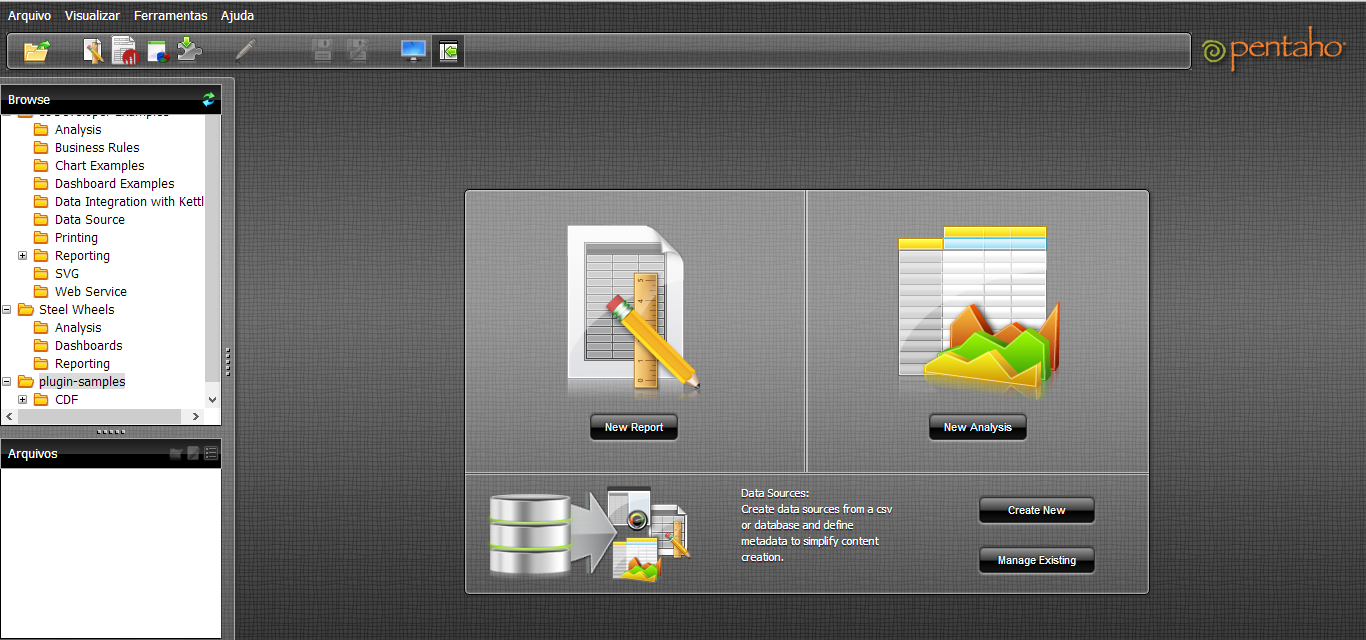
\includegraphics[keepaspectratio=false,scale=0.45]{figuras/pentahoBI.eps}
\caption{Interface do Pentaho BI Platform}
\label{BIplatform}
\end{figure}
\FloatBarrier
 

A ferramenta Pentaho BI Platform como a infraestrutura do ambiente de \textit{Data Warehousing}, possui arquitetura extensível por plugins diversos que realizam diversas operações, tais como, criação de relatórios, visualização dos dados em tabelas e gráficos e entre outros. Entre os plugins disponíveis, está o Saiku Analitics que oferece serviços de apoio a operações OLAP e à visualização de dados. As características gerais do Saiku Analitics, bem como a avaliação quanto aos critérios gerais de seleção de ferramentas, são apresentados na Tabela \ref{saiku}. 

\begin{table}[!ht]
\begin{tabular}{|p{4.5cm}|p{5.0cm}|p{1cm}|p{1cm}|p{1cm}|p{1cm}|}
\hline
Característica                                          

&


\begin{center}

\includegraphics[keepaspectratio=false,scale=0.4]{figuras/saiku_olap_logo.eps} 
\end{center}                                              

& CG01 

& CG02       

& CG03       


& CG04       


\\ \hline

Licença                                                 & GPL 2.0                              & \checkmark &            &            &            \\ \hline
Componentes de Visualização                           & Tabelas e Gráficos &            &            &            &            \\ \hline
Gráficos com Suporte & Gráfico de Pizza, Gráfico de Linhas, Gráfico de Área, Gráfico de Setor e entre outros &            &            &            &

 \\ \hline
Ultima Versão Estável (14/11/2013)                      & 2.5                                             &            &            &            & \checkmark \\ \hline
Quantidade de Commits no Repositório Oficial em 14/11/2013            & 790                                         &            &            & \checkmark &            \\ \hline
Idioma da Documentação                                  & Inglês                                          &            & \checkmark &            &            \\ \hline            
Quantidade de Casos Abertos no \textit{Issue Tracker} & 227                                           &&            & \checkmark &            \\ \hline

\end{tabular}
\caption{Características do Saiku Analytics e avaliação quanto aos critérios gerais de seleção de ferramentas}
\label{saiku}
\end{table}
\FloatBarrier


O Saiku Analytics, tem em sua arquitetura, um outro componente da arquitetura do Pentaho BI Suite, que é o Mondrian OLAP Server. Este permite ao Saiku, que sejam realizadas consultas \textit{ad hoc} com as dimensões do cubo, de um esquema dimensional, realizando \textit{drag and drop} das colunas das dimensões.

Há também, a possibilidade, da realização de consultas por meio da escrita de \textit{queries} em linguagem MDX \textit{(MulitDimensional eXpressions)}. Esta foi proposta por \citeonline{spofford2006mdx} como uma forma de escrever consultas mais otimizadas para bases seguem o modelo dimensional, tal como mostra o trecho de Código-Fonte \ref{MDX}.




\begin{center}
\begin{minipage}{0.5\textwidth}

\begin{lstlisting}[caption=Exemplo de \textit{Query} em linguagem MDX, label=MDX]
 SELECT
   { [Measures].[Loja] } ON COLUMNS,
   { [Tempo].[2002], [Tempo].[2003] } ON ROWS
FROM Vendas
WHERE ( [Loja].[Loja Sul]) 

\end{lstlisting}
\end{minipage}
\end{center}
\FloatBarrier


Após a carga das métricas de código-fonte do projeto Apache Maven no \textit{data warehouse} foi possível então realizar a implementação de algumas consultas OLAP, \textit{ad hoc}, para eventual visualização de dados em tabela e gráficos tal como mostra a Figura \ref{table} e a Figura \ref{chart}. 



\begin{figure}[ht!]
\centering
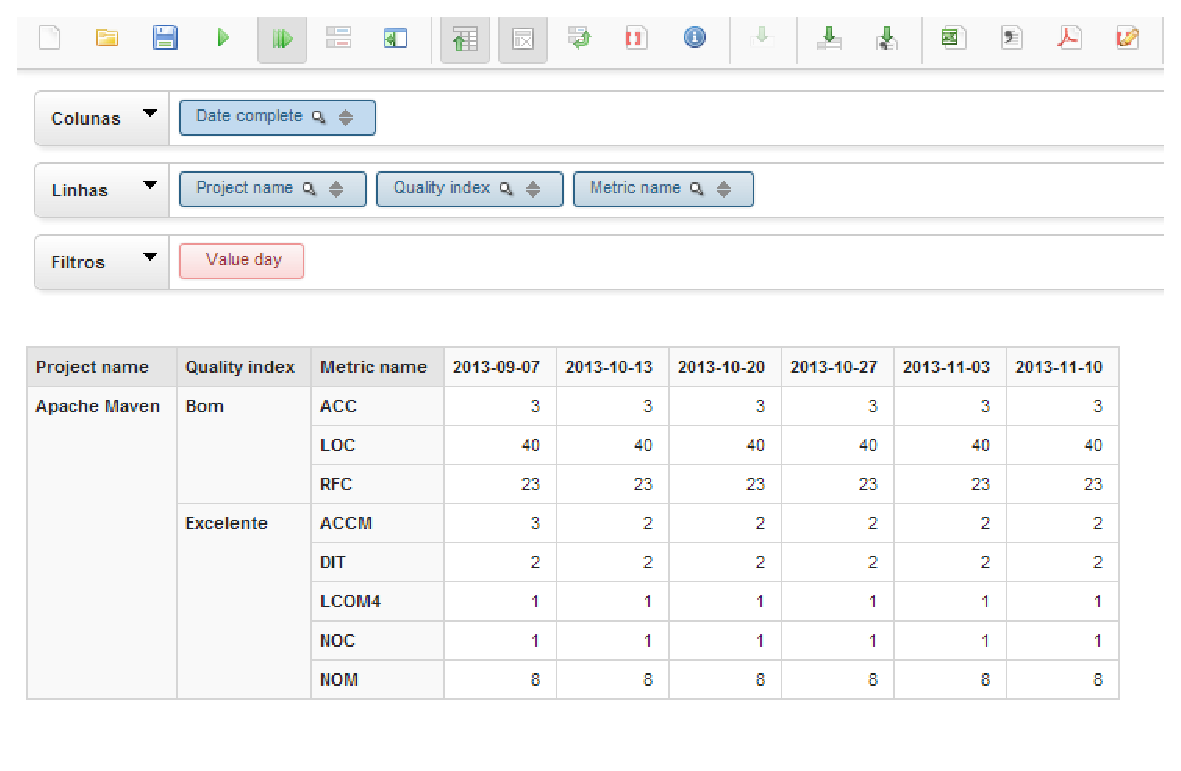
\includegraphics[keepaspectratio=false,scale=0.83]{figuras/indicadores.eps}
\caption{Visualização de dados do Apache Maven em formato de tabela no Saiku Analytics}
\label{table}
\end{figure}
\FloatBarrier
 



\begin{figure}[ht!]
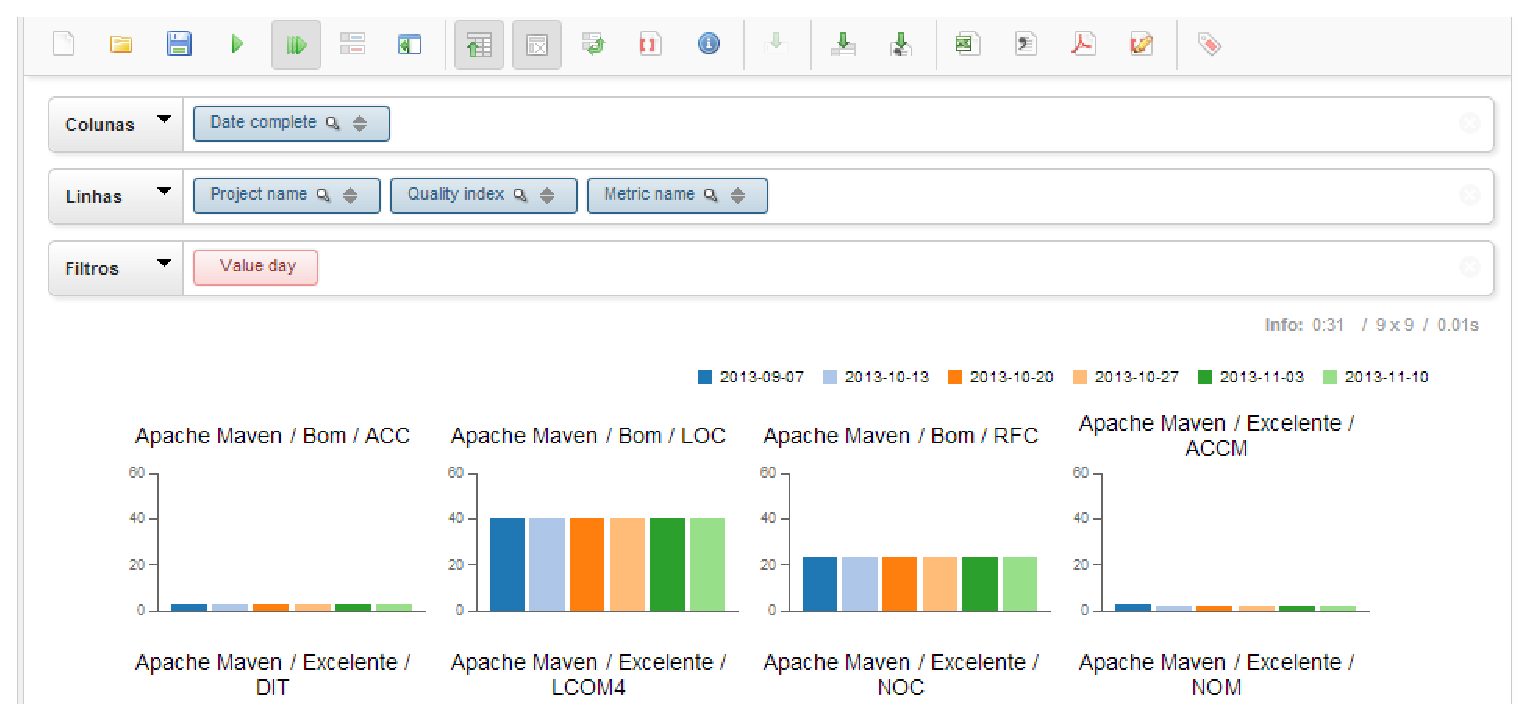
\includegraphics[keepaspectratio=false,scale=0.63]{figuras/indicadores_graficos.eps}
\caption{Visualização de dados do Apache Maven em formato de gráfico de barras no Saiku Analytics}
\label{chart}
\end{figure}
\FloatBarrier
 
